% ======================================================================
% scrjura-en.tex
% Copyright (c) Markus Kohm, 2011-2022
%
% This file is part of the LaTeX2e KOMA-Script bundle.
%
% This work may be distributed and/or modified under the conditions of
% the LaTeX Project Public License, version 1.3c of the license.
% The latest version of this license is in
%   http://www.latex-project.org/lppl.txt
% and version 1.3c or later is part of all distributions of LaTeX 
% version 2005/12/01 or later and of this work.
%
% This work has the LPPL maintenance status "author-maintained".
%
% The Current Maintainer and author of this work is Markus Kohm.
%
% This work consists of all files listed in MANIFEST.md.
% ======================================================================
%
% Chapter about scrjura of the KOMA-Script guide
% Maintained by Markus Kohm
%
% ======================================================================

\KOMAProvidesFile{scrjura-en.tex}%
                 [$Date: 2022-06-05 12:40:11 +0200 (So, 05. Jun 2022) $
                  KOMA-Script guide (chapter: scrjura)]

\translator{Alexander Willand\and Markus Kohm\and Karl Hagen}

\chapter{Support for the Law Office with \Package{scrjura}}
\labelbase{scrjura}
\BeginIndexGroup
\BeginIndex{Package}{scrjura}

If you want to write a contract\Index{contract}, the articles of association
for a company or an association, a law, or a legal commentary, the package
\Package{scrjura} will provide typographical support. Although
\Package{scrjura} is intended to provide general help for legal documents, the
contract is the central element of the package. Particular attention is paid
to clauses, titles, and numbered provisions\,---\,if there are several of
them in a clause\,---, numbered sentences, entries in the table of
contents, and cross references according to German standards.

The package has been developed in cooperation with Dr Alexander Willand of
Karlsruhe. Many of its features go back to constructive inquiries from Prof
Heiner Richter of the Hochschule Stralsund University of Applied Sciences.

Note\textnote{Attention!} that the package works with
\Package{hyperref}\IndexPackage{hyperref}. Nevertheless, \Package{hyperref}
has to be loaded after \Package{scrjura} as usual.

\LoadCommonFile{options}% \section{Early or late Selection of Options}

\LoadCommonFile{textmarkup}% \section{Text Markup}

\section{Table of Contents}
\seclabel{toc}

The headings of clauses can also be added automatically to the table of
contents, if desired.
% TODO: Fix new translation
Therefore\ChangedAt{v3.27}{\Package{scrjura}} the package uses
\DescRef{tocbasic.cmd.DeclareTOCStyleEntry}\IndexCmd{DeclareTOCStyleEntry}
(see \autoref{sec:tocbasic.tocstyle},
\DescPageRef{tocbasic.cmd.DeclareTOCStyleEntry}) to define an \PName{entry
  level} named \PValue{cpar}.
% :ODOT


\begin{Declaration}
  \OptionVName{juratotoc}{simple switch}%
  \OptionVName{juratotoc}{level number}
\end{Declaration}
Clauses\Index{clause} are shown in the table of contents only if their
\PName{level number} is less than or equal to the
\DescRef{maincls.counter.tocdepth}%
\important{\DescRef{maincls.counter.tocdepth}}\IndexCounter{tocdepth} counter
(see \autoref{sec:maincls.toc}, \DescPageRef{maincls.counter.tocdepth}). By
default, the \PName{level number} is \Length{maxdimen}, which is also used if
the option is switched off with the \PName{simple
  switch}\important{\OptionValue{juratotoc}{false}} (see
\autoref{tab:truefalseswitch}, \autopageref{tab:truefalseswitch}). Because the
\DescRef{maincls.counter.tocdepth} counter usually has a one-digit value,
clause entries are therefore not normally displayed in the table of contents.

If you switch on the option using the \PName{simple switch}%
\important{\OptionValue{juratotoc}{true}}, the \PName{level number} 2 is used
so that clauses are shown in the table of contents on the same level as
subsections. For the default setting of \DescRef{maincls.counter.tocdepth},
clauses are then shown in all \KOMAScript{} classes.

% TODO: Fix new translation
Internally\ChangedAt{v3.27}{\Package{scrjura}} usage of this option results in
a call of
\DescRef{tocbasic.cmd.DeclareTOCStyleEntry}\IndexCmd{DeclareTOCStyleEntry}
with the \PName{style} \PValue{default} and a corresponding value of
\Option{level} in the \PName{option list}.%
% :ODOT
\EndIndexGroup


\begin{Declaration}
  \OptionVName{juratocindent}{indent}%
  \OptionVName{juratocnumberwidth}{number width}
\end{Declaration}
These two options can be used to determine the indentation for the clause
entries in the table of contents as well as the space reserved for the numbers
there. The defaults are the same as for subsection entries in
\Class{scrartcl}.

% TODO: Fix new translation
Internally\ChangedAt{v3.27}{\Package{scrjura}} usage of these options results
in calls of
\DescRef{tocbasic.cmd.DeclareTOCStyleEntry}\IndexCmd{DeclareTOCStyleEntry}
with the \PName{style} \PValue{default} and \OptionVName{indent}{indent}
respectively \OptionVName{numwidth}{number width} in the \PName{option list}.%
% :ODOT
\EndIndexGroup


\section{Environment for Contracts}
\seclabel{contract}

\BeginIndexGroup
\BeginIndex{}{contract}
The essential mechanisms of \Package{scrjura} are available only inside the
contract environment.

\begin{Declaration}
  \begin{Environment}{contract}\end{Environment}
\end{Declaration}
Currently, this is the one and only environment for \Package{scrjura}. Using
it activates automatic numbering of paragraphs and the
\DescRef{\LabelBase.cmd.Clause} and \DescRef{\LabelBase.cmd.SubClause}
commands, which will be documented below, are given concrete form.

The\textnote{Attention!} \DescRef{\LabelBase.env.contract} environment must
not be nested within itself. Within a document, however, you can use the
environment several times. The clauses within these environments are treated
as if they were within a single environment. As a result, ending the
environment really only temporarily interrupts it, and the old environment is
continued by the beginning of a new environment. However, you cannot end the
environment within a clause.%
\EndIndexGroup


\begin{Declaration}
  \Option{contract}
\end{Declaration}
The whole document becomes a contract if you use this option while loading the
package with \DescRef{\LabelBase.cmd.usepackage}%
\important{\DescRef{\LabelBase.cmd.usepackage}} or as a global option with
\DescRef{\LabelBase.cmd.documentclass}%
\important{\DescRef{\LabelBase.cmd.documentclass}}. The document then behaves
exactly as if it contained one \DescRef{\LabelBase.env.contract} environment.

Note\textnote{Attention!} that you cannot set the \Option{contract} option
with \DescRef{\LabelBase.cmd.KOMAoption} or
\DescRef{\LabelBase.cmd.KOMAoptions}. Thus you cannot switch the option off
again. Instead, you should use a \DescRef{\LabelBase.env.contract} environment
directly.%
\EndIndexGroup


\subsection{Clauses}
\label{sec:scrjura.clause}
\index{section|seealso{clause}}

Clauses\footnote{%
  In English, a ``clause'' in a legal document is a section, paragraph, or
  phrase that relates to a particular point. Although it is common in English
  to also use the terms ``article'' or ``section'' for what we here call a
  ``clause'', we use the latter term throughout to avoid confusion with the
  \Class{article} class and the \DescRef{maincls.cmd.section} and
  \DescRef{maincls.cmd.paragraph} sectioning divisions of most document
  classes.} in a legal sense are defined in \Package{scrjura} only within
contracts, that is inside the \DescRef{\LabelBase.env.contract} environment or
other environments declared with
\DescRef{\LabelBase.cmd.DeclareNewJuraEnvironment} (see
\autoref{sec:\LabelBase.newenv},
\DescPageRef{\LabelBase.cmd.DeclareNewJuraEnvironment}).

\begin{Declaration}
  \Macro{Clause}\OParameter{options}%
  \Macro{SubClause}\OParameter{options}
\end{Declaration}
These are the most important commands inside of a contract. Without using any
additional \PName{options}, \Macro{Clause} creates the heading of a clause,
which consists of the sign ``\S'', followed by its number. In contrast,
\Macro{SubClause} creates the heading of a clause with the last number used by
\Macro{Clause} and adds a lower-case letter. \Macro{SubClause} is mainly
intended for cases where an act or a contract is amended and not only are
clauses changed or deleted but new clauses are inserted between existing ones
without completely changing the numbering.

Both commands accept a a comma-separated list of \PName{options}. An overview
of the available properties is shown in \autoref{tab:scrjura.Clause.options}.
The most important of them will be discussed in more detail.

\begin{table}
  \caption{Available properties for the optional argument of \Macro{Clause} and
    \Macro{SubClause}}
  \label{tab:scrjura.Clause.options}
  \begin{desctabular}
    \entry{\Option{dummy}}{%
      The heading will not be printed but is counted in the automatic
      numbering.%
    }%
    \entry{\OptionVName{head}{running head}}{%
      If running heads are active, this \PName{running head} is used instead of
      the clause \PName{title}.%
    }%
    \entry{\Option{nohead}}{%
      The running head stays unchanged.%
    }%
    \entry{\Option{notocentry}}{%
      Does not make an entry into the table of contents.%
    }%
    \entry{\OptionVName{number}{number}}{%
      Uses \PName{number} for the output of the clause number.%
    }%
    \entry{\OptionVName{preskip}{skip}}{%
      Changes the vertical \PName{skip} before the clause heading.%
    }%
    \entry{\OptionVName{postskip}{skip}}{%
      Changes the vertical \PName{skip} after the clause heading.%
    }%
    \entry{\OptionVName{title}{title}}{%
      The clause \PName{title} will be printed in addition to the clause
      number. This is also used as the default for the \PName{running head}
      and the \PName{entry} in the table of contents.%
    }%
    \entry{\OptionVName{tocentry}{entry}}{%
      Regardless of the clause \PName{title}, an \PName{entry} into the
      table of contents will be made, if such entries are activated.%
    }%
  \end{desctabular} 
\end{table}

By default, a skip of two lines is inserted before the heading and a skip of
one line afterwards. You can change the size of these skips with the
\Option{preskip}\important[i]{\Option{preskip}, \Option{postskip}} and
\Option{postskip} options. The new values apply  not only to the current
clause but from the current clause until the end of the current contract
environment. You can also make the appropriate settings in advance with
\begin{flushleft}\quad\small
  \textbf{\Macro{setkeys}}\PParameter{contract}%
  \PParameter{preskip=\PName{skip},\\
    \normalsize\quad\small
    \hspace{11.5em}postskip=\PName{skip}}
\end{flushleft}
regardless of the specific clause and outside of a contract environment. You
can also set these options inside the preamble after loading
\Package{scrjura}, but you cannot set them while loading the package or by
using \DescRef{\LabelBase.cmd.KOMAoptions} or
\DescRef{\LabelBase.cmd.KOMAoption}.

\BeginIndex{FontElement}{contract.Clause}\LabelFontElement{contract.Clause}%
\BeginIndex{FontElement}{Clause}\LabelFontElement{Clause}%
By default, clause headings use the font style
\Macro{sffamily}\Macro{bfseries}\Macro{large}. You can change this font style
at any time using the
\FontElement{contract.Clause}\important{\FontElement{contract.Clause}} element
with \DescRef{\LabelBase.cmd.setkomafont}%
\important[i]{\DescRef{\LabelBase.cmd.setkomafont},
\DescRef{\LabelBase.cmd.addtokomafont}} and
\DescRef{\LabelBase.cmd.addtokomafont} (see \autoref{sec:maincls.textmarkup},
\DescPageRef{\LabelBase.cmd.setkomafont}). Inside the
\DescRef{\LabelBase.env.contract} environment, you can also use
\FontElement{Clause}\important{\FontElement{Clause}} instead of
\FontElement{contract.Clause}.%
\EndIndex{FontElement}{Clause}%
\EndIndex{FontElement}{contract.Clause}

With the \Option{title}\important[i]{\Option{title}, \Option{head},
  \Option{tocentry}}, \Option{head}, and \Option{tocentry} options, you can
title a clause in addition to the number. You\textnote{Attention!} should put
the value of each options inside curly brackets. Otherwise, for example,
commas which are meant to be part of the value will be confused with the
delimiters between different options. Empty values for \Option{head} and
\Option{tocentry} cause empty entries. If you want to avoid an entry, use the
\Option{nohead}\important[i]{\Option{nohead}, \Option{notocentry}} and
\Option{notocentry} options.

Instead of consecutive numbers, you can also set a clause number manually with
the \Option{number}\important{\Option{number}} option. However, this does not
affect the numbers of the subsequent clauses. Empty numbers are not possible.
Fragile commands inside \PName{number} have to be protected with
\Macro{protect}. You\textnote{Attention!} should use only numbers and letters
as a \Option{number}.

With the \Option{dummy}\important{\Option{dummy}} option, you can suppress the
output of the whole heading of a clause. The automatic numbering, however,
will still count this clause. In this way, you can skip an automatically
numbered clause with\textnote{Example}
\begin{lstcode}
  \Clause{dummy}
\end{lstcode}
in case the clause corresponding clause has been deleted in a later version of
a contract.

Note\textnote{Attention!} that the \Option{dummy} option only accepts the
values \PValue{true} and \PValue{false}. All other values are usually ignored,
but can lead to an error message in the worst case scenario.%
\EndIndexGroup


\begin{Declaration}
  \Macro{Clauseformat}\Parameter{number}
\end{Declaration}
As already mentioned, clauses and subclauses are normally numbered. The number
is formatted with the help of the \Macro{Clauseformat} command, which expects
the number as the only argument. The default is the following:
\begin{lstcode}
  \newcommand*{\Clauseformat}[1]{\S~#1}
\end{lstcode}
This produces the section mark, \Macro{S}\IndexCmd{S} (\S), followed by a
non-breaking space and the number. If you redefine this command, be sure it
remains expandable.%
\EndIndexGroup


\begin{Declaration}
  \OptionVName{juratitlepagebreak}{simple switch}
\end{Declaration}%
Usually, page breaks are prohibited within heading of all kinds. However, some
lawyers require page breaks within clause headings. You can allow such a break
by using \Option{juratitlepagebreak}\important{\Option{juratitlepagebreak}}.
You can find the available values for \PName{simple switch} in
\autoref{tab:truefalseswitch}, \autopageref{tab:truefalseswitch}.%
\EndIndexGroup
  
\begin{Declaration}
  \OptionVName{clausemark}{value}
\end{Declaration}%
Since clauses are a subordinate structure with independent numbering, they do
not produce running heads by default. You can, however, create running heads
with various settings. You can find the available \PName{values} and their
meanings in \autoref{tab:scrjura.clausemark}.%
%
\begin{table}
  \caption{Available values for the \Option{clausemark} option to activate
    running heads}%
  \label{tab:scrjura.clausemark}%
  \begin{desctabular}
    \entry{\PValue{both}}{%
      Clauses generate left and right marks for running heads, if the document
      provides automatic running heads.%
      \IndexOption{clausemark~=\textKValue{both}}%
    }%
    \entry{\PValue{false}, \PValue{off}, \PValue{no}}{%
      Clauses do not generate marks for running heads and therefore do not
      change running heads.%
      \IndexOption{clausemark~=\textKValue{false}}%
    }%
    \entry{\PValue{forceboth}}{%
      Clauses use \DescRef{maincls.cmd.markboth} to generate left and right
      marks for running heads even if the document does not provide automatic
      running heads for the current page style.%
      \IndexOption{clausemark~=\textKValue{forceboth}}%
    }%
    \entry{\PValue{forceright}}{%
      Clauses use \DescRef{maincls.cmd.markright} to generate right marks for
      running heads even if the document does not provide automatic running
      heads for the current page style.%
      \IndexOption{clausemark~=\textKValue{forceright}}%
    }%
    \entry{\PValue{right}}{%
      Clauses generate right marks for running heads, if the document provides
      automatic running heads.%
      \IndexOption{clausemark~=\textKValue{right}}%
    }%
  \end{desctabular}
\end{table}
%
\EndIndexGroup


\subsection{Paragraphs}
\label{sec:scrjura.par}
\BeginIndexGroup
\BeginIndex{}{paragraph>numbering}%
Within clauses, \Package{scrjura} usually numbers paragraphs automatically.
With this, the paragraphs provide a powerful structuring element, similar to
\DescRef{maincls.cmd.paragraph} or \DescRef{maincls.cmd.subparagraph} in
normal documents. For this reason, contracts usually use a vertical skip
between paragraphs. The \Package{scrjura} package does not provide its own
mechanism for this. Instead, it uses the \DescRef{maincls.option.parskip}%
\IndexOption{parskip}\important{\DescRef{maincls.option.parskip}} option of
the \KOMAScript{} classes (see \autoref{sec:maincls.parmarkup},
\DescPageRef{maincls.option.parskip}).


\begin{Declaration}
  \OptionVName{parnumber}{value}
\end{Declaration}
The default numbering of paragraphs is \OptionValue{parnumber}{auto} and
\OptionValue{parnumber}{true}. Sometimes you may need to disable the automatic
numbering. You can do this with \OptionValue{parnumber}{false}%
\important{\OptionValue{parnumber}{false}}%
\IndexOption{parnumber~=\textKValue{false}}. In this case, only the sentence
numbering is reset.

To implement this option, it has been necessary to hook into the
paragraph-building mechanism of \LaTeX. In some rare cases, this can have a
negative effect. If so, you can undo the change with
\OptionValue{parnumber}{manual}%
\important{\OptionValue{parnumber}{manual}}%
\IndexOption{parnumber~=\textKValue{manual}}. On the other hand, \LaTeX{}
itself sometimes undoes the change. In those cases you can activate it again
with \OptionValue{parnumber}{auto}%
\important{\OptionValue{parnumber}{auto}}%
\IndexOption{parnumber~=\textKValue{auto}}.

Clauses that consist of a single paragraph do not automatically receive a
paragraph number. For this to work, there must not be two clauses with an
identical number in a document. However should you ever need such numbering,
you should switch to another contract environment (see
\DescRef{\LabelBase.cmd.DeclareNewJuraEnvironment},
\autoref{sec:\LabelBase.newenv},
\DescPageRef{\LabelBase.cmd.DeclareNewJuraEnvironment}).
Note\textnote{Attention!} that the number of paragraphs in a clause is not
available before the end of the clause. Therefore you need a least two
\LaTeX{} runs before the automatic paragraph numbering is correct.%
\EndIndexGroup


\begin{Declaration}
  \Counter{par}%
  \Macro{thepar}%
  \Macro{parformat}%
  \Macro{parformatseparation}
\end{Declaration}%
For numbering the paragraphs inside a clause we use the \Counter{par} counter.
The output of \Macro{thepar} will display an Arabic number, because the
default is \Macro{arabic}\PParameter{par}. \Macro{parformat} provides the
format, which is \Macro{thepar} in rounded brackets. When numbering a
paragraph manually, you should also use \Macro{parformat}. It makes sense to
call \Macro{parformat} with a subsequent \Macro{parformatseparation}, or at
least a \Macro{nobreakspace} or tilde.

With\ChangedAt{v0.7}{\Package{scrjura}} automatic numbering, \Macro{parformat}
is followed by \Macro{parformatseparation}, which currently consists of
\Macro{nonbreakspace}, the non-breakable space.

\BeginIndex{FontElement}{parnumber}\LabelFontElement{parnumber}%
The paragraph number is usually printed using the currently active font.
However, you can change this default for the \FontElement{parnumber} element
at any time with \DescRef{\LabelBase.cmd.setkomafont}%
\important[i]{\DescRef{\LabelBase.cmd.setkomafont},
\DescRef{\LabelBase.cmd.addtokomafont}} and
\DescRef{\LabelBase.cmd.addtokomafont} (see
\autoref{sec:\LabelBase.textmarkup},
\DescPageRef{\LabelBase.cmd.setkomafont}).%
\EndIndex{FontElement}{parnumber}%

Note\textnote{Attention!} that \Package{scrjura} assumes internally that
\Macro{thepar} is an Arabic number. Therefore you should definitely not
redefine it!%
\EndIndexGroup


\begin{Declaration}
  \Macro{withoutparnumber}
\end{Declaration}
If the paragraph number is not printed, \Package{scrjura} executes the
\Macro{withoutparnumber} command at the beginning of the new paragraph. The
initial definition of this command is empty. This means it is a kind of dummy
command that does nothing. It has been implemented because of a user request.
Most users can ignore this command.%
\EndIndexGroup


\begin{Declaration}
  \Macro{ellipsispar}\OParameter{number}%
  \Macro{parellipsis}
\end{Declaration}
Sometimes\ChangedAt{v0.7}{\Package{scrjura}}\,---\,particularly in comparative
commentaries\,---\,it is desirable to omit paragraphs but to mark the
omission. Those omitted paragraphs\Index{paragraph>omission} should be taken
into account by the paragraph counter. The package \Package{scrjura} provides
the command \Macro{ellipsispar} to do this.

By default, \Macro{ellipsispar} omits precisely one paragraph. Using the
optional argument, you can omit multiple paragraphs. In any case, the output
shows just one unnumbered paragraph, which consists only of the ellipsis
defined by \Macro{parellipsis}. The automatic numbering of paragraphs takes
the \PName{number} of omitted paragraphs into account.
\begin{Example}
  Suppose you are writing a comment on the German\footnote{Please remember,
    this translation does not refer to an existing law but is only an example
    of how you might realise such a commentary with \Package{scrjura}.} penal
  code, but only on paragraph 3 of \S~2. Nevertheless, you'd like to indicate
  the omission indirectly. You can do this with:
\begin{lstcode}
  \documentclass[parskip=half]{scrartcl}
  \usepackage{scrjura}
  \begin{document}
  \begin{contract}
    \Clause{title={Temporal application},number=2}
    \ellipsispar[2]

    If the law that applies at the time the criminal act is
    committed is changed before the verdict, then the most
    lenient law shall be applicable.

    \ellipsispar[3]
  \end{contract}
  \end{document}
\end{lstcode}
  To see the result, just give it a try.
\end{Example}

The ellipsis is by default \Macro{textellipsis}\IndexCmd{textellipsis}, if
such a command is defined. If not, \Macro{dots} is used. You can redefine
\Macro{parellipsis} at any time with \Macro{renewcommand}.%
\EndIndexGroup
%
\EndIndexGroup


\subsection{Sentences}
\label{sec:scrjura.sentence}

\BeginIndexGroup%
\BeginIndex{}{sentence>number}%
Paragraphs in contracts consist of one or more sentences, some of which may
also be numbered. However, as automatic numbering is cumbersome and
error-prone, it has not yet been implemented in
\Package{scrjura}. Semi-automatic numbering, however, is supported.

\begin{Declaration}
  \Counter{sentence}
  \Macro{thesentence}
  \Macro{sentencenumberformat}
  \Macro{Sentence}
\end{Declaration}
Manual numbering of sentences is done with the \Macro{Sentence} command. It
adds one to the \Counter{sentence} counter. By default,
\Macro{sentencenumberformat}\ChangedAt{v3.26}{\Package{scrjura}} prints
\Macro{thesentence} as an Arabic number in superscript.

\BeginIndex{FontElement}{sentencenumber}\LabelFontElement{sentencenumber}%
The\ChangedAt{v3.26}{\Package{scrjura}} sentence number is usually printed
using the currently active font.  However, you can change this default for the
\FontElement{parnumber} element at any time with
\DescRef{\LabelBase.cmd.setkomafont}%
\important[i]{\DescRef{\LabelBase.cmd.setkomafont},
  \DescRef{\LabelBase.cmd.addtokomafont}} and
\DescRef{\LabelBase.cmd.addtokomafont} (see
\autoref{sec:\LabelBase.textmarkup},
\DescPageRef{\LabelBase.cmd.setkomafont}).%
\EndIndex{FontElement}{sentencenumber}%

Using\textnote{Hint!} \Package{babel}\IndexPackage{babel} offers an easy way
to define a shorthand for \Macro{Sentence}:%
\phantomsection\label{sec:scrjura.shorthandexample}%
\begin{lstcode}[moretexcs={useshorthands,defineshorthand}]
  \useshorthands{'}
  \defineshorthand{'S}{\Sentence\ignorespaces}
\end{lstcode}
With this definition, any space after \lstinline|'S| will be ignored. You can
even use the dot as an abbreviation for a dot and a new sentence number:
\begin{lstcode}[moretexcs={useshorthands,defineshorthand}]
  \defineshorthand{'.}{. \Sentence\ignorespaces}
\end{lstcode}
For details regarding \Macro{useshorthands} and \Macro{defineshorthands},
please consult the manual of the \Package{babel} package (see
\cite{package:babel}). You can find an example of their application in
\autoref{sec:scrjura.example}, \autopageref{sec:scrjura.example}.%
\EndIndexGroup
%
\EndIndexGroup
%
\EndIndexGroup


\section{Cross-References}
\seclabel{ref}

The conventional mechanism to set cross-references using
\Macro{label}\IndexCmd{label}\important{\Macro{label}}, \Macro{ref}, and
\Macro{pageref} does not suffice for clauses, paragraphs, and sentences.
Therefore \Package{scrjura} provides additional commands.

\begin{Declaration}
  \Macro{ref}\Parameter{label}%
  \Macro{refL}\Parameter{label}%
  \Macro{refS}\Parameter{label}%
  \Macro{refN}\Parameter{label}
\end{Declaration}
The commands \Macro{refL}, \Macro{refS}, and \Macro{refN} give a full
reference to clause, paragraph and sentence. \Macro{refL} is a long text,
\Macro{refS} a short text, and \Macro{refN} an abbreviated, numeric form.
\Macro{ref} defaults to \Macro{refL}.%
\EndIndexGroup


\begin{Declaration}
  \Macro{refClause}\Parameter{label}%
  \Macro{refClauseN}\Parameter{label}
\end{Declaration}
These commands reference a clause without displaying the paragraph or
sentences. \Macro{refClause} puts a section mark (\S) in front of the
reference, while \Macro{refClauseN} does not.%
\EndIndexGroup


\begin{Declaration}
  \Macro{refPar}\Parameter{label}%
  \Macro{refParL}\Parameter{label}%
  \Macro{refParS}\Parameter{label}%
  \Macro{refParN}\OParameter{number format}\Parameter{label}
\end{Declaration}
You can reference just a paragraph with \Macro{refParL}, \Macro{refParS} and
\Macro{refParN}. The differences between the forms correspond to the
differences between \DescRef{\LabelBase.cmd.refL},
\DescRef{\LabelBase.cmd.refN} and \DescRef{\LabelBase.cmd.refS}. A feature
worth noting is the optional argument of \Macro{refParN}. Usually the numeric
reference to a paragraph uses a Roman number. You can, however, specify a
different \PName{number format} in the optional argument. This option
primarily makes sense to use Arabic numbers. By default, \Macro{refPar} is
\Macro{refParL}.%
\EndIndexGroup


\begin{Declaration}
  \Macro{refSentence}\Parameter{label}%
  \Macro{refSentenceL}\Parameter{label}%
  \Macro{refSentenceS}\Parameter{label}%
  \Macro{refSentenceN}\Parameter{label}
\end{Declaration}
You can reference a sentence with \Macro{refSentenceL}, \Macro{refSentenceS},
or \Macro{refSentenceN}. Again, there is a long text form, a short text form,
and a numerical form. By default, \Macro{refSentence} is
\Macro{refSentenceL}.%
\EndIndexGroup


\begin{Declaration}
  \OptionVName{ref}{value}
\end{Declaration}
The results of \DescRef{\LabelBase.cmd.ref}, \DescRef{\LabelBase.cmd.refPar},
and \DescRef{\LabelBase.cmd.refSentence} depend on the \PName{value} of the
\Option{ref} option. The defaults are \DescRef{\LabelBase.cmd.refL},
\DescRef{\LabelBase.cmd.refParL} and \DescRef{\LabelBase.cmd.refSentenceL}.
You can find the available values and their meaning in
\autoref{tab:scrjura.ref}.%
%
\begin{table}
%\begin{desclist}
%  \desccaption
  \caption[{%
    Available values for the \Option{ref} option to configure the
    cross-reference format%
  }]{%
    Available values for the \Option{ref} option to configure the
    cross-reference format of \DescRef{\LabelBase.cmd.ref},
    \DescRef{\LabelBase.cmd.refPar}, and \DescRef{\LabelBase.cmd.refSentence}%
    \label{tab:scrjura.ref}%
  }%
  \begin{desctabular}
    \entry{\PValue{long}}{%
      A combination of \PValue{parlong} and \PValue{sentencelong}.%
      \IndexOption{ref~=\textKValue{long}}%
    }%
    \entry{\PValue{numeric}}{%
      A combination of \PValue{parnumeric} and \PValue{sentencenumeric}.%
      \IndexOption{ref~=\textKValue{numeric}}%
    }%
    \entry{\PValue{clauseonly}, \PValue{onlyclause}, \PValue{ClauseOnly},
      \PValue{OnlyClause}}{%
      A combination of \PValue{paroff} and \PValue{sentenceoff}. Note that
      \DescRef{\LabelBase.cmd.refPar} and \DescRef{\LabelBase.cmd.refSentence}
      produce empty results!%
      \IndexOption{ref~=\textKValue{long}}%
    }%
    \entry{\PValue{parlong}, \PValue{longpar}, \PValue{ParL}}{%
      Paragraphs are referenced in long textual form.%
      \IndexOption{ref~=\textKValue{parlong}}%
    }%
    \entry{\PValue{parnumeric}, \PValue{numericpar}, \PValue{ParN}}{%
      Paragraphs are referenced in simple numerical form.%
      \IndexOption{ref~=\textKValue{parnumeric}}%
    }%
    \entry{\PValue{paroff}, \PValue{nopar}}{%
      Paragraphs have no reference. Note that \DescRef{\LabelBase.cmd.refPar}
      produces an empty result!%
      \IndexOption{ref~=\textKValue{paroff}}%
    }%
    \entry{\PValue{parshort}, \PValue{shortpar}, \PValue{ParS}}{%
      Paragraphs are referenced in short textual form.%
      \IndexOption{ref~=\textKValue{parshort}}%
    }%
    \entry{\PValue{sentencelong}, \PValue{longsentence}, \PValue{SentenceL}}{%
      Sentences are referenced in long textual form.%
      \IndexOption{ref~=\textKValue{parlong}}%
    }%
    \entry{\PValue{sentencenumeric}, \PValue{numericsentence},
      \PValue{SentenceN}}{%
      Sentences are referenced in simple numeric form.%
      \IndexOption{ref~=\textKValue{sentencenumeric}}%
    }%
    \entry{\PValue{sentenceoff}, \PValue{nosentence}}{%
      Sentences have no reference. Note that
      \DescRef{\LabelBase.cmd.refSentence} produces an empty result!%
      \IndexOption{ref~=\textKValue{sentenceoff}}%
    }%
    \entry{\PValue{sentenceshort}, \PValue{shortsentence},
      \PValue{SentenceS}}{%
      Sentences are referenced in short textual form.%
      \IndexOption{ref~=\textKValue{sentenceshort}}%
    }%
    \entry{\PValue{short}}{%
      A combination of \PValue{parshort} and \PValue{sentenceshort}.%
      \IndexOption{ref~=\textKValue{value}}%
    }%
\end{desctabular}
\end{table}

\begin{Example}
  Suppose you always want to reference paragraphs in the form ``paragraph 1
  in clause 1''. As there is no predefined command for this, you have
  to create your own definition from the available options. You can achieve
  this easily with:%
\begin{lstcode}
  \newcommand*{\refParM}[1]{%
    paragraph~\refParN[arabic]{#1} 
    in clause~\refClauseN{#1}%
  }
\end{lstcode}
  This new command can be used in the same way as
  \DescRef{\LabelBase.cmd.refParL}.%
\end{Example}%

You can find examples of results of the basic commands in
\autoref{tab:scrjura.refexamples}.%
%
\begin{table}
  \KOMAoptions{captions=topbeside}%
  \setcapindent{0pt}%
  \begin{captionbeside}{Example outputs of the \Option{ref}-independent 
    cross-reference commands}[l]
    \begin{tabular}[t]{ll}
      \toprule
      Command                               & Example output \\
      \midrule
      \DescRef{\LabelBase.cmd.refL}\Parameter{label}           & \S{} 1 paragraph 1 sentence 1 \\
      \DescRef{\LabelBase.cmd.refS}\Parameter{label}           & \S{} 1 par. 1 sent. 1 \\
      \DescRef{\LabelBase.cmd.refN}\Parameter{label}           & \S{} 1 I 1. \\
      \DescRef{\LabelBase.cmd.refClause}\Parameter{label}   & \S{} 1 \\
      \DescRef{\LabelBase.cmd.refClauseN}\Parameter{label}  & 1 \\
      \DescRef{\LabelBase.cmd.refParL}\Parameter{label}        & paragraph 1 \\
      \DescRef{\LabelBase.cmd.refParS}\Parameter{label}        & par. 1 \\
      \DescRef{\LabelBase.cmd.refParN}\Parameter{label}        & I \\
      \DescRef{\LabelBase.cmd.refParN}\POParameter{arabic}\Parameter{label} & 1 \\
      \DescRef{\LabelBase.cmd.refParN}\POParameter{roman}\Parameter{label} & i \\
      \DescRef{\LabelBase.cmd.refSentenceL}\Parameter{label}   & sentence 1 \\
      \DescRef{\LabelBase.cmd.refSentenceS}\Parameter{label}   & sent. 1 \\
      \DescRef{\LabelBase.cmd.refSentenceN}\Parameter{label}   & 1. \\
      \bottomrule
   \end{tabular}
  \end{captionbeside}
  \label{tab:scrjura.refexamples}
\end{table}
\EndIndexGroup


\section{Additional Environments}
\seclabel{newenv}

Some users do not use \Package{scrjura} to draft contracts or commentaries on
individual laws but to examine different types of laws, which may not
necessarily use the section prefix (\S) before the title of each clause but
perhaps something like ``Art.'' or ``IAS'', and so forth. An independent
counter is also required for each of these different clause types.

\begin{Declaration}
  \Macro{DeclareNewJuraEnvironment}\Parameter{name}\OParameter{options}%
  \Parameter{start commands}\Parameter{end commands}
\end{Declaration}
You\ChangedAt{v0.9}{\Package{scrjura}} can use this command to define new and
independent environments for contracts or other legal texts. The argument
\PName{name} is the name of the new environment, of course. The \PName{start
commands} are commands which will be executed at the beginning of the
environment, as if they were added directly after
\Macro{begin}\Parameter{name}. Correspondingly \PName{end commands} will be
executed at the end of the environment, as if added directly before
\Macro{end}\Parameter{name}. Without any \PName{options} the new environment
behaves like the \DescRef{\LabelBase.env.contract} environment, but with its
own counters. It is possible to set \PName{options} in a comma-separated list.
See \autoref{tab:\LabelBase.DeclareNewJuraEnvironment} for the currently
supported \PName{options}.

\begin{desclist}
  \desccaption{Options provided by \Macro{DeclareNewJuraEnvironment} for new
    contract environments\label{tab:\LabelBase.DeclareNewJuraEnvironment}}%
  {Options of \Macro{DeclareNewJuraEnvironment} (\emph{continued})}%
  \entry{\OptionVName{Clause}{command}}{%
    Defines the \PName{command} to which the \DescRef{\LabelBase.cmd.Clause}
    command is mapped within the environment. This \PName{command}, like the
    one documented for \DescRef{\LabelBase.env.contract}, expects exactly one
    argument. To use it correctly requires advanced knowledge of the
    \Package{scrjura}'s internal functioning. Furthermore, the requirements
    for the \PName{command} may change in future versions. Therefore it is
    recommended not to use this option!%
  }%
  \entry{\OptionVName{ClauseFont}{commands}}{%
    \leavevmode\BeginIndex{FontElement}{\PName{Name}.Clause}%
    \LabelFontElement{\PName{Name}.Clause}%
    If this option is used, a new
    \FontElement{\PName{Name}.Clause}\IndexFontElement{\PName{Name}.Clause}
    element is defined using
    \DescRef{maincls-experts.cmd.newkomafont}\IndexCmd{newkomafont}, with the
    \PName{commands} used as its default setting. If the element was
    previously defined as an alias (see
    \DescRef{maincls-experts.cmd.aliaskomafont} in
    \autoref{sec:maincls-experts.fonts},
    \DescPageRef{maincls-experts.cmd.aliaskomafont}), it will become an
    independent element instead. If it has already been defined as an
    independent element, \DescRef{\LabelBase.cmd.setkomafont} is used to set
    the \PName{commands} a new font settings. Please note the limitations for
    font settings in \autoref{sec:\LabelBase.textmarkup},
    \DescPageRef{\LabelBase.cmd.setkomafont}.
    \EndIndex{FontElement}{\PName{Name}.Clause}%
  }%
  \entry{\OptionVName{SubClause}{command}}{%
    Defines the \PName{command} to which the
    \DescRef{\LabelBase.cmd.SubClause} command is mapped within the
    environment. This \PName{command}, like the one documented for
    \DescRef{\LabelBase.env.contract}, expects exactly one argument. To use it
    correctly requires advanced knowledge of the \Package{scrjura}'s internal
    functioning. Furthermore, the requirements for the \PName{command} may
    change in future versions. Therefore it is recommended not to use this
    option!%
  }%
  \entry{\OptionVName{Sentence}{command}}{%
    Defines the \PName{command} to which the 
    \DescRef{\LabelBase.cmd.Sentence} is mapped within the environment. This
    \PName{command} must not have an argument. Typically it should add one to
    the  \Counter{sentence}\IndexCounter{sentence} (using
    \Macro{refstepcounter}\IndexCmd{refstepcounter}) counter and display it
    appropriately. It is particularly important to avoid adding unwanted
    spaces.%
  }%
  \entry{\OptionVName{ClauseNumberFormat}{command}}{%
    Formats the numbers of clauses within the environment. The \PName{command}
    should expect exactly one argument: the number of the clause. If the
    \PName{command} implements a series of commands and the number is the last
    argument of a that series, you can directly use the series of commands as
    \PName{command}.%
  }
\end{desclist}
\begin{Example}
  To define the environment for articles we mentioned in the preface of this
  section, it is sufficient to write:
\begin{lstcode}
  \DeclareNewJuraEnvironment{Article}[ClauseNumberFormat=Art.~]{}{}
\end{lstcode}
  If we are using a \KOMAScript{} class and want to separate the paragraphs in
  this environment with space instead of using paragraph indentation, we can
  use:
\begin{lstcode}
  \DeclareNewJuraEnvironment{Article}[ClauseNumberFormat=Art.~]
                            {\KOMAoptions{parskip}}{}
\end{lstcode}
  In cross-references, ``Art.'' will  of course be used instead of ``\S''.%

  The new environment is used like \DescRef{\LabelBase.env.contract}:
\begin{lstcode}
  \begin{Article}
    \Clause{}
    Human dignity is inviolable. To respect and protect people is a
    duty of all state authority.
  \end{Article}
\end{lstcode}
\end{Example}%
\EndIndexGroup


\section{Support for Different Languages}
\seclabel{babel}

The \Package{scrjura} package has been developed in cooperation with a German
lawyer. Therefore it initially supported only the languages \PValue{german},
\PValue{ngerman}, \PValue{austrian}, and \PValue{naustrian}. Nevertheless, it
has been designed to support common language packages like
\Package{babel}\important{\Package{babel}}\IndexPackage{babel}. Users can
easily make changes by using \DescRef{scrbase.cmd.providecaptionname} (see
\autoref{sec:scrbase.languageSupport},
\DescPageRef{scrbase.cmd.providecaptionname}). If you have definitive
information about the correct legal terms and conventions of a language,
please contact the \KOMAScript{} author. Support for English has been added in
this way, and so \Package{scrjura} now also provides terms for the languages
\PValue{english}, \PValue{american}, \PValue{british}, \PValue{canadian},
\PValue{USenglish}, and \PValue{UKenglish}.

\begin{Declaration}
  \Macro{parname}%
  \Macro{parshortname}%
  \Macro{sentencename}%
  \Macro{sentenceshortname}
\end{Declaration}
These are the language-dependent terms used by \Package{scrjura}. The meaning
of the terms and their English defaults are shown in
\autoref{tab:scrjura.captionnames}. The package itself defines them by using
\DescRef{scrbase.cmd.providecaptionname} inside
\Macro{begin}\PParameter{document} only if other requirements have not already
been met. If you use \Package{scrjura} with an unsupported language, the
package will throw an error.%
%
\begin{table}
  \KOMAoptions{captions=topbeside}%
  \setcapindent{0pt}%
  \begin{captionbeside}
    [{%
      Meanings and English defaults of language-dependent terms%
    }]{%
      Meanings and English defaults of language-dependent terms, if not
      already defined%
    } [l]
    \begin{tabular}[t]{lll}
      \toprule
      Command                   & Meaning                   & Default \\
      \midrule
      \Macro{parname}           & long form ``paragraph''   & paragraph \\
      \Macro{parshortname}      & short form ``paragraph''  & par. \\
      \Macro{sentencename}      & long form ``sentence''    & sentence \\
      \Macro{sentenceshortname} & short form ``sentence''   & sent. \\
      \bottomrule
    \end{tabular}
  \end{captionbeside}
  \label{tab:scrjura.captionnames}
\end{table}
%
\EndIndexGroup


\section{A Detailed Example}
\seclabel{example}

You may remember the letter from \autoref{cha:scrlttr2}, in which  a club
member wanted to remind the board about an overdue meeting that was prescribed
by the club's by-laws. Such club by-laws are a kind of contract, and you can
create them using \Package{scrjura}.

\lstinputcode[{xleftmargin=2em,%
  linerange=1-2}]{scrjura-example-en.tex}%
We use class \Class{scrartcl}. Because paragraph distance instead of paragraph
indentation is usual in club by-laws, we load the class with option
\OptionValueRef{maincls}{parskip}{half} (see \autoref{sec:maincls.parmarkup},
\DescPageRef{maincls.option.parskip}).

\lstinputcode[{xleftmargin=2em,%
  linerange=4-4}]{scrjura-example-en.tex}%
The club rules are in British English. Therefore we load the \Package{babel}
package with the \Option{british} option too.

\iffree{%
\lstinputcode[{xleftmargin=2em,%
  linerange={6-6,8-8}}]{scrjura-example-en.tex}%
}{%
\lstinputcode[{xleftmargin=2em,%
  linerange={6-6,9-9}}]{scrjura-example-en.tex}%
}%
We make some default font settings. Earlier versions of the example also
loaded the \Package{textcomp} package here for an improved section mark
(\S). Since \LaTeX{} 2020/02/01, however, the desired functionality is directly
integrated in the \LaTeX{} kernel.

\lstinputcode[{xleftmargin=2em,%
  linerange=11-11}]{scrjura-example-en.tex}%
Later in the document, we want lists numbered not with Arabic numbers but with
lower-case letters. We can do this easily with the \Package{enumerate}
package. Alternatively, we could have used the \Package{enumitem} package.

\lstinputcode[{moretexcs={useshorthands,defineshorthand},%
  xleftmargin=2em,%
  linerange=13-21}]{scrjura-example-en.tex}%
Now it is time for \Package{scrjura}. The
\OptionValueRef{\LabelBase}{clausemark}{forceboth} option forces clauses to
create left and right marks for the running head. On the other hand, we do not
want \DescRef{maincls.cmd.section} to change the marks for the running head.
Therefore we use the \PageStyle{myheadings} page style. This page style
generally does not provide automatic running heads.

Later, we also want a table of contents with the clauses. This can be achieved
with the \DescRef{\LabelBase.option.juratotoc} option. Doing so we will see
that the default width for these numbers is insufficient for the clause
numbers in the table of contents. With
\OptionValueRef{\LabelBase}{juratocnumberwidth}{2.5em}, we reserve more space.

The definition of shorthands has already been explained in
\autoref{sec:scrjura.shorthandexample}. In this example we do the same thing
to simplify the input.

\lstinputcode[{xleftmargin=2em,%
  linerange=23-23}]{scrjura-example-en.tex}%
It is time to begin the actual document.

\lstinputcode[{xleftmargin=2em,%
  linerange=25-29}]{scrjura-example-en.tex}%
Like other documents, the by-laws have a title. We created it with the usual
\KOMAScript{} commands (see \autoref{sec:maincls.titlepage}, starting on
\autopageref{sec:maincls.titlepage}).

\lstinputcode[{xleftmargin=2em,%
  linerange=31-31}]{scrjura-example-en.tex}%
As already mentioned, we want to create a table of contents.

\lstinputcode[{xleftmargin=2em,%
  linerange=33-37}]{scrjura-example-en.tex}%
Preambles are not unusual in club by-laws. Here we use
\DescRef{maincls.cmd.addsec} to create one because we want it to have an entry
in the table of contents.

\lstinputcode[{xleftmargin=2em,%
  linerange=39-39}]{scrjura-example-en.tex}%
Here we use a small trick. The articles of the club by-laws should be numbered
with upper-case letters instead of Arabic numbers, just as 
the appendix sections of an article using \Class{scrartcl} are.

\lstinputcode[{xleftmargin=2em,%
  linerange=41-43}]{scrjura-example-en.tex}%
We begin the contract with the first article.

\lstinputcode[{xleftmargin=2em,%
  linerange=44-54}]{scrjura-example-en.tex}%
The first clause has a number and a title. We will do the same with all
following clauses.

The first paragraph of the clause contains nothing unusual. Because it is not
the only paragraph, every paragraph will be automatically preceded by a
paragraph number. Note that the numbering the first paragraph requires at
least two \LaTeX{} runs. Since this is the case for the table of contents as
well, this does not create any additional problems.

In the second paragraph we have two sentences. Here we can see the shorthands
\texttt{'S} and \texttt{'.} in action. The first one only generates the
sentence number. The second one generates not only the full stop but also the
sentence number. With this, both sentences are numbered.

\lstinputcode[{xleftmargin=2em,%
  linerange=55-70}]{scrjura-example-en.tex}%
The second clause: again this contains several paragraphs, some of which
include several sentences. The second paragraph also has a numbered list. In
the last paragraph, we set a label, because we want to reference it later.

\lstinputcode[{xleftmargin=2em,%
  linerange=72-78}]{scrjura-example-en.tex}%
The third clause contains something special: a cross-reference. Here we use
the long form with clause, paragraph, and sentence. If we decided later that
sentences should not be included in the reference, we could use the
\OptionValueRef{\LabelBase}{ref}{nosentence} option to set this globally.

\lstinputcode[{xleftmargin=2em,%
  linerange=80-81}]{scrjura-example-en.tex}%
Here we have a special kind of clause. In earlier versions of the club by-laws,
this was a real clause, but it was later removed. However, the
numbering of the following clauses should not be changed by removing this
one. Therefore the \DescRef{\LabelBase.cmd.Clause} statement has not been
removed but supplemented by option \Option{dummy}. With this, we also can set
a label even though the clause will not be printed.

\lstinputcode[{xleftmargin=2em,%
  linerange=82-86}]{scrjura-example-en.tex}%
Another article begins. To avoid problems with the paragraph numbering, we
interrupt the \DescRef{\LabelBase.env.contract} environment.

\lstinputcode[{xleftmargin=2em,%
  linerange=87-87}]{scrjura-example-en.tex}%
The first clause of the next article also has been deleted.

\lstinputcode[{xleftmargin=2em,%
  linerange=89-98}]{scrjura-example-en.tex}%
Here we have a real clause again. We cross-reference one of the deleted
clauses and also set a label.

\lstinputcode[{xleftmargin=2em,%
  linerange=100-104}]{scrjura-example-en.tex}%
Once more, this is a special kind of clause. This time we have not removed a
clause but added one without renumbering the following clauses. To do so,
we use \DescRef{\LabelBase.cmd.SubClause}. Therefore the clause number is the
same like the previous one but with an appended ``a''.

\lstinputcode[{xleftmargin=2em,%
  linerange=106-126}]{scrjura-example-en.tex}%
The other clauses of this article are very usual. You already know all the
features used for them.

\lstinputcode[{xleftmargin=2em,%
  linerange=128-141}]{scrjura-example-en.tex}%
There follows another article no special features.

\lstinputcode[{xleftmargin=2em,%
  linerange=143-143}]{scrjura-example-en.tex}%
Then the \LaTeX{} document ends. You can see first three pages in
\autoref{fig:scrjura.example}.%
%
\begin{figure}
  \setcapindent{0pt}%
  \iffree{%
    {\hfill
      \frame{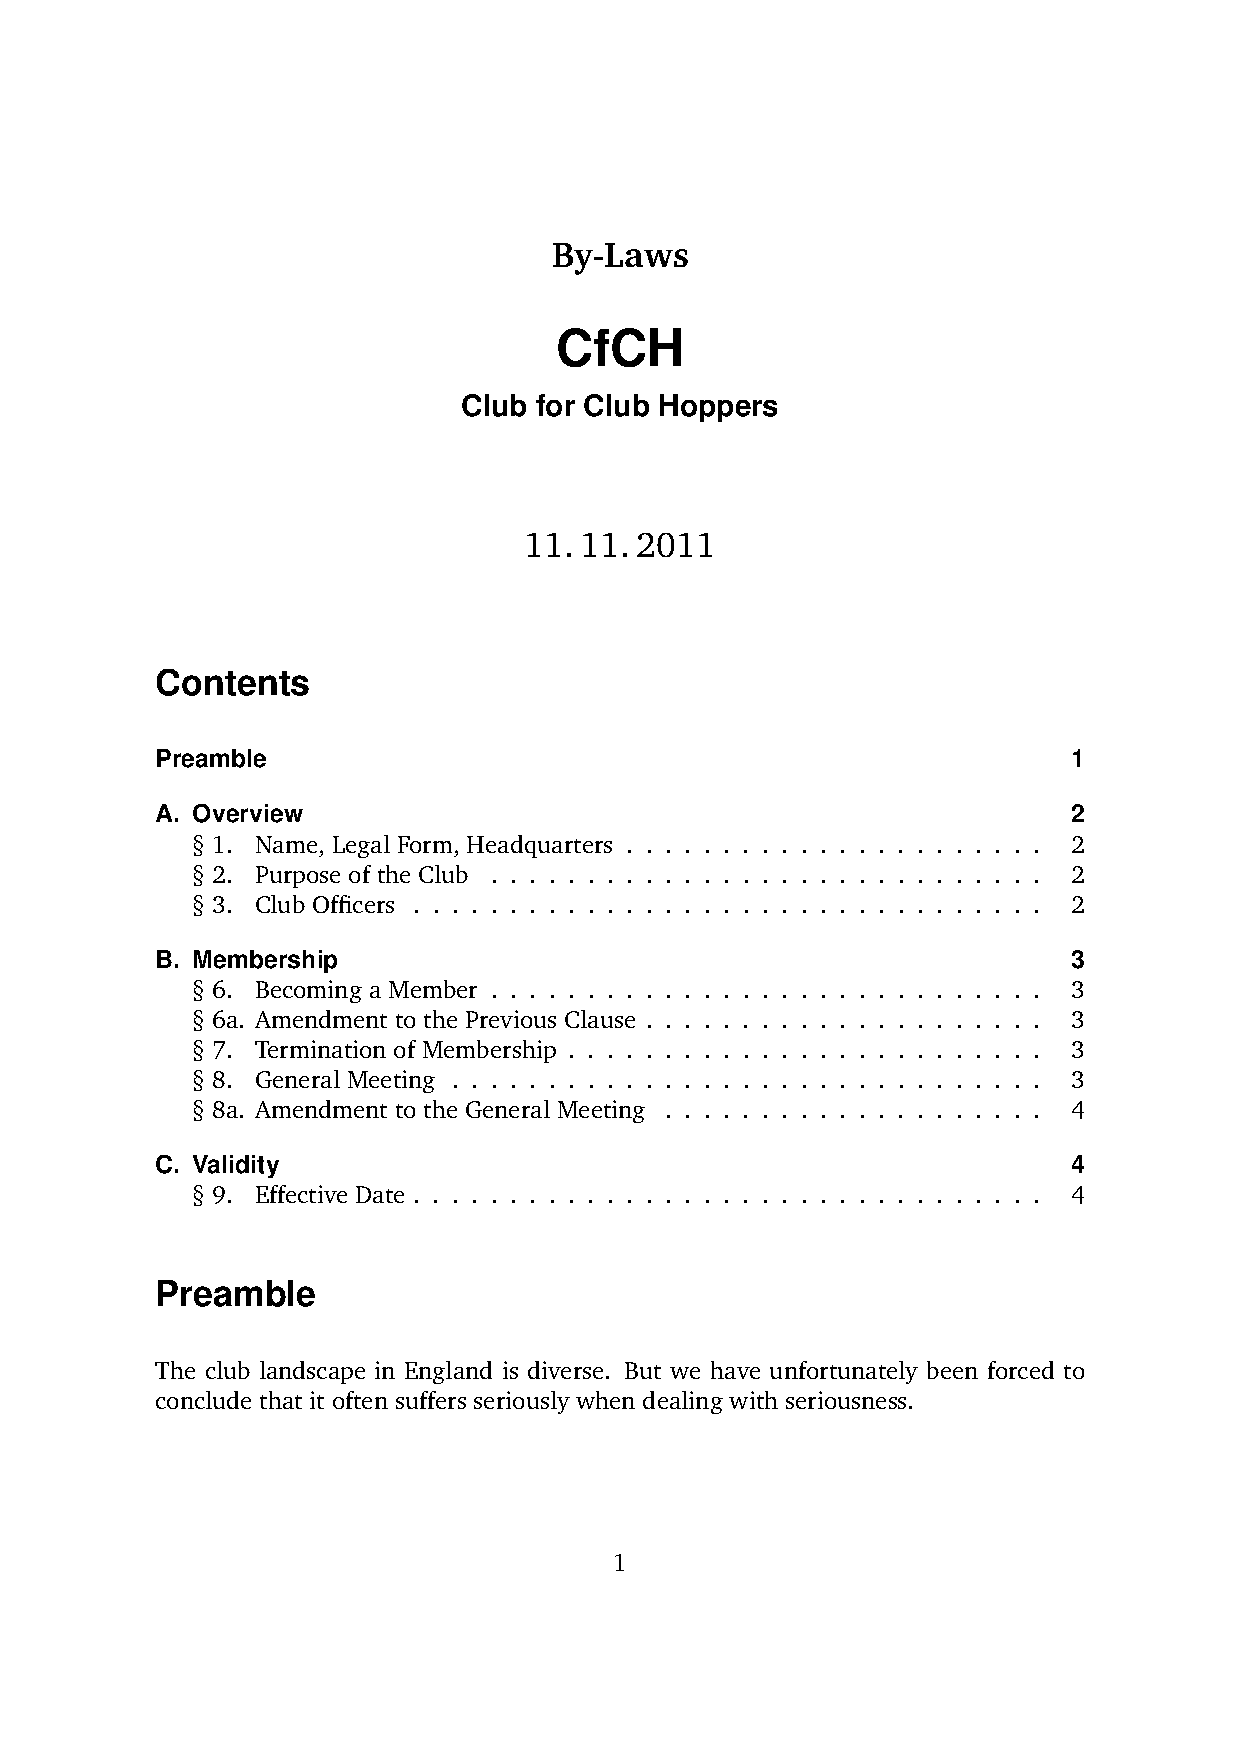
\includegraphics[page=1,width=.482\textwidth,%
        height=.49\textheight,keepaspectratio]{scrjura-example-en}}\enskip
      \frame{\includegraphics[page=2,width=.482\textwidth,%
        height=.49\textheight,keepaspectratio]{scrjura-example-en}}\par
      \smallskip}
    \begin{captionbeside}[{%
        Example: First three pages of the example club by-laws of
        \protect\autoref{sec:scrjura.example}%
      }]{%
        First three pages of the example club by-laws of
        \protect\autoref{sec:scrjura.example}%
      }%
      [l]
      \frame{\includegraphics[page=3,width=.482\textwidth,%
        height=.49\textheight,keepaspectratio]{scrjura-example-en}}\enskip
    \end{captionbeside}
  }{%
    {\hfill
      \frame{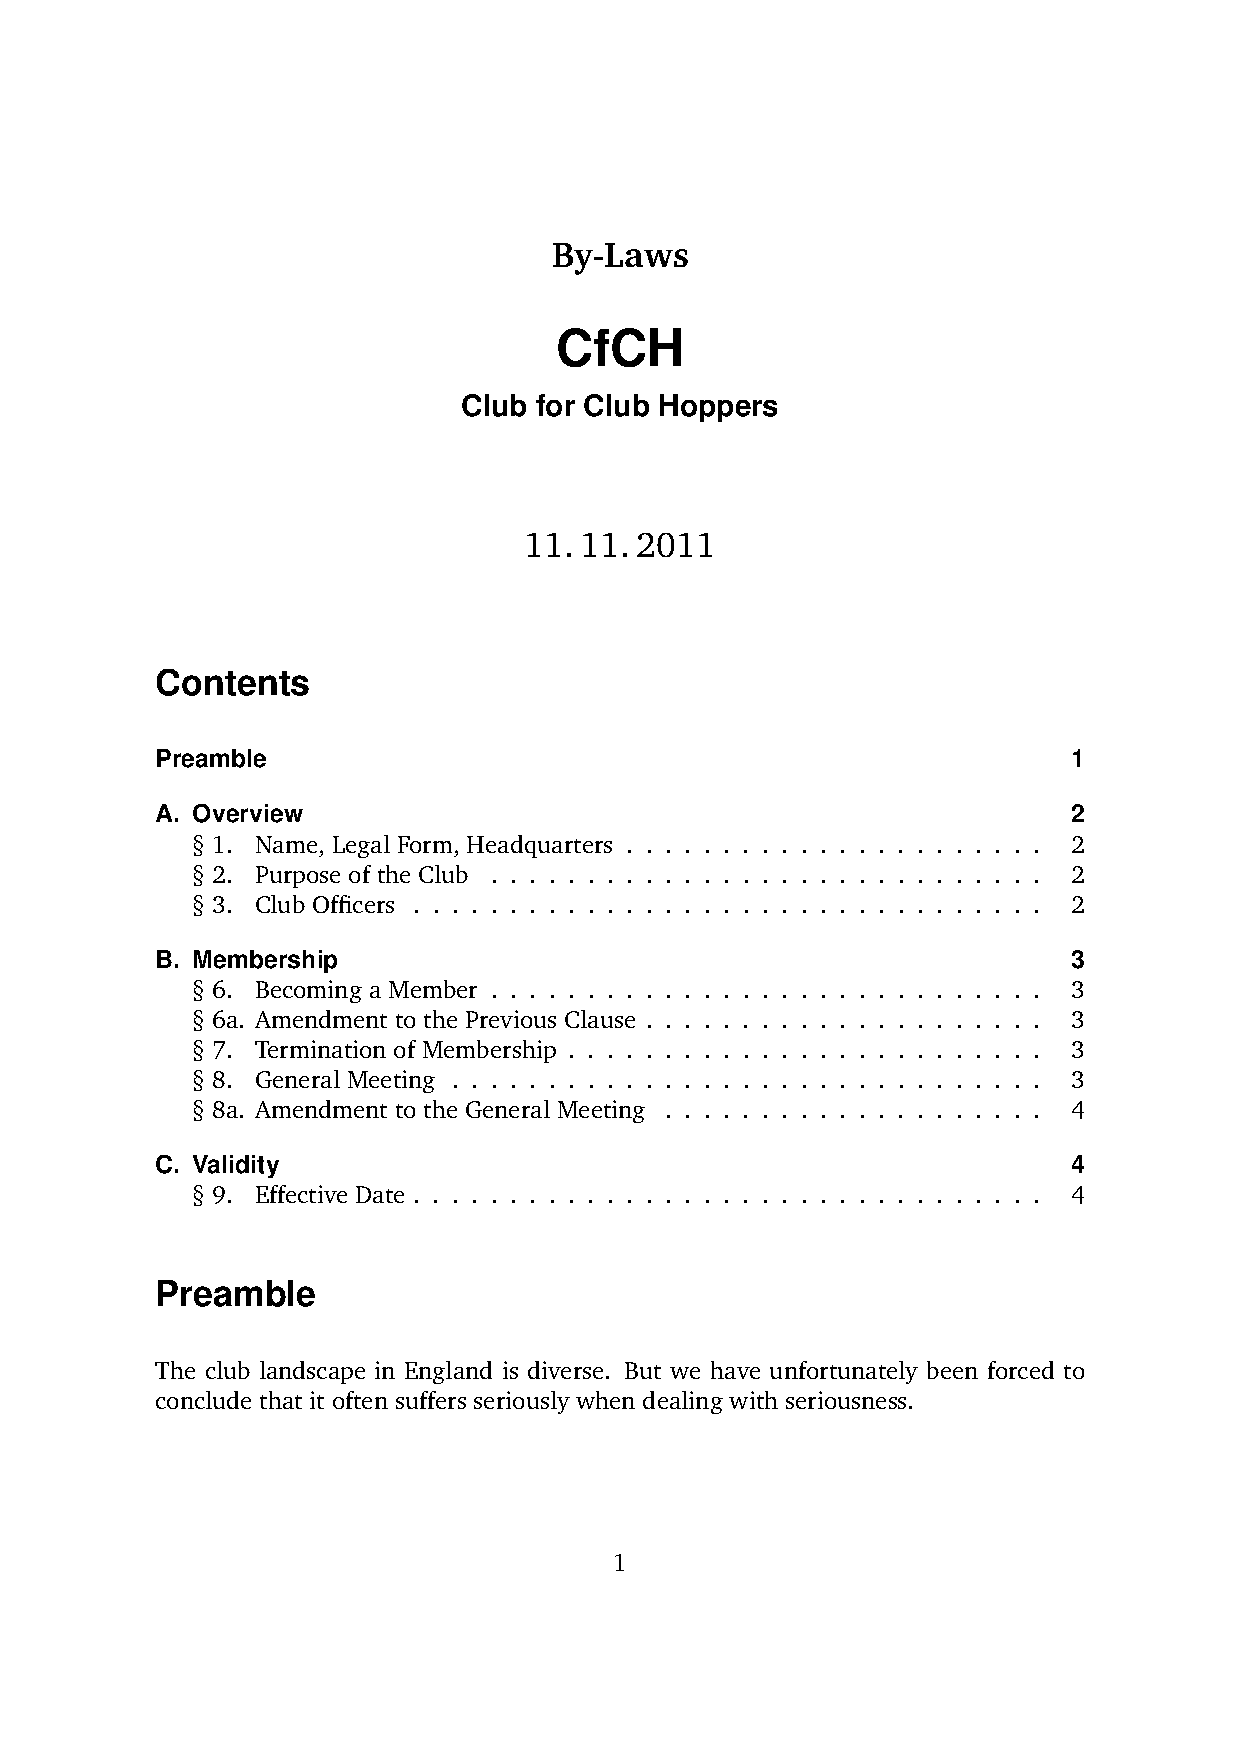
\includegraphics[page=1,width=.482\textwidth]{scrjura-example-en}}%
      \enskip
      \frame{\includegraphics[page=2,width=.482\textwidth]{scrjura-example-en}}\par
      \smallskip}
    \begin{captionbeside}[{%
        Example: First three pages of the example club by-laws of
        \protect\autoref{sec:scrjura.example}%
      }]{%
        First three pages of the example club by-laws of
        \protect\autoref{sec:scrjura.example}%
      }%
      [l]
      \frame{\includegraphics[page=3,width=.482\textwidth]{scrjura-example-en}}%
      \enskip
    \end{captionbeside}
  }%
  \label{fig:scrjura.example}
\end{figure}

\section{State of Development}
\seclabel{draft}

Since \KOMAScript~3.24, the \Package{scrjura} package has shared the version
number of the classes and other important packages of \KOMAScript.
Nevertheless, you should note that so far, the interaction of the
\DescRef{\LabelBase.env.contract} environment with the many different settings
possible with other \LaTeX{} environments, packages, or classes has not been
tested. The main reason for this is that \Package{scrjura} is very specialised
and far beyond the author's ordinary practice. So the author mostly relies on
detailed user feedback.%
\EndIndexGroup

\endinput

%%% Local Variables: 
%%% mode: latex
%%% TeX-master: "scrguide-en.tex"
%%% coding: utf-8
%%% ispell-local-dictionary: "en_GB"
%%% eval: (flyspell-mode 1)
%%% End: 
